\documentclass[aspectratio=169,10pt]{beamer}

% Compile from the folder that contains ultrasound-beamforming-benchmarks/ :
%   pdflatex -interaction=nonstopmode -halt-on-error beamforming_project.tex
% The cyst plot is looked up in ultrasound-beamforming-benchmarks/results/plots/ and ../results/plots/.
% If it is missing, a labelled empty box is drawn instead of failing.

\usepackage[T1]{fontenc}
\usepackage[utf8]{inputenc}
\usepackage{lmodern}
\usepackage{amsmath,amssymb,booktabs,graphicx,tabularx,array,xcolor,listings,tikz}
\usetikzlibrary{arrows.meta,calc,positioning}

\definecolor{Ink}{HTML}{1E2A36}
\definecolor{Navy}{HTML}{1F3A5F}
\definecolor{Accent}{HTML}{0B6E8A}
\definecolor{Muted}{HTML}{66727D}
\definecolor{Rule}{HTML}{C9D1D8}
\definecolor{LightBg}{HTML}{EEF2F5}
\definecolor{Warn}{HTML}{A33A3A}

\usetheme{default}
\setbeamertemplate{navigation symbols}{}
\setbeamercolor{normal text}{fg=Ink,bg=white}
\setbeamercolor{structure}{fg=Accent}
\setbeamercolor{frametitle}{fg=Navy}
\setbeamerfont{frametitle}{size=\Large,series=\bfseries}
\setbeamertemplate{frametitle}{%
  \vspace{.3cm}{\usebeamercolor[fg]{frametitle}\usebeamerfont{frametitle}\insertframetitle\par}%
  \vspace{.05cm}{\color{Rule}\rule{\textwidth}{.6pt}}}
\setbeamertemplate{itemize item}{\raise.15ex\hbox{\color{Accent}\scriptsize$\bullet$}}
\setbeamertemplate{enumerate item}{\color{Accent}\insertenumlabel.}
\setbeamertemplate{blocks}[default]
\setbeamercolor{block title}{fg=Accent,bg=LightBg}
\setbeamercolor{block body}{fg=Ink,bg=LightBg}
\setbeamerfont{block title}{size=\normalsize,series=\bfseries}
\setbeamersize{text margin left=.8cm,text margin right=.8cm}
\setbeamertemplate{footline}{%
  \leavevmode\hbox to\paperwidth{\hspace{.8cm}\color{Muted}\scriptsize
  Ultrasound beamforming: DAS and DMAS on CPU and GPU\hfill\insertframenumber\hspace{.8cm}}\vskip.3cm}

\lstset{basicstyle=\ttfamily\small,commentstyle=\color{Muted},showstringspaces=false,
  columns=fullflexible,keepspaces=true,backgroundcolor=\color{LightBg},frame=none}

\newcommand{\plot}[1]{%
  \IfFileExists{ultrasound-beamforming-benchmarks/results/plots/#1}%
   {\includegraphics[width=\linewidth,height=.5\textheight,keepaspectratio]{ultrasound-beamforming-benchmarks/results/plots/#1}}%
   {\IfFileExists{../results/plots/#1}%
     {\includegraphics[width=\linewidth,height=.5\textheight,keepaspectratio]{../results/plots/#1}}%
     {\fbox{\parbox[c][.4\textheight][c]{.9\linewidth}{\centering\tiny plot not found}}}}}

\begin{document}

% 1 -------------------------------------------------------------- title
\begin{frame}[plain]
  \vspace*{1.3cm}
  \hspace*{.9cm}\begin{minipage}{.85\textwidth}
    {\color{Accent}\small\bfseries Sem 7 project}\par\vspace{.7em}
    {\color{Navy}\fontsize{26}{30}\selectfont\bfseries Ultrasound beamforming:\\ DAS and DMAS on CPU and GPU\par}
    \vspace{.6em}
    {\color{Muted}\large Making the computation faster without changing the beamforming model\par}
    \vspace{1.2cm}
    {\small [Team member names]\par [Course name, institute]}
  \end{minipage}
\end{frame}

% 2 -------------------------------------------------------------- problem
\begin{frame}{Problem statement}
  \begin{columns}[T,onlytextwidth]
    \column{.54\textwidth}
    A linear array records echoes on 128 channels after each of 21 plane-wave transmissions. The scanner stores raw RF traces; the image has to be computed from them.

    \medskip
    For every pixel, the beamformer works out when its echo reaches each channel, reads the sample at that time, and combines the values.
    \column{.4\textwidth}
    \begin{block}{Size of the computation}
      \small
      \begin{tabularx}{\linewidth}{@{}l r r@{}}
        Grid & Pixels & Terms\\\midrule
        $128\times191$ & 24,448 & 65.7 M\\
        $507\times600$ & 304,200 & 817.7 M\\
      \end{tabularx}\\[.3em]
      \scriptsize terms = pixels $\times$ 21 $\times$ 128
    \end{block}
  \end{columns}
\end{frame}

% 3 -------------------------------------------------------------- DAS
\begin{frame}{Delay-and-sum (DAS)}
  \begin{columns}[T,onlytextwidth]
    \column{.4\textwidth}
    \centering
    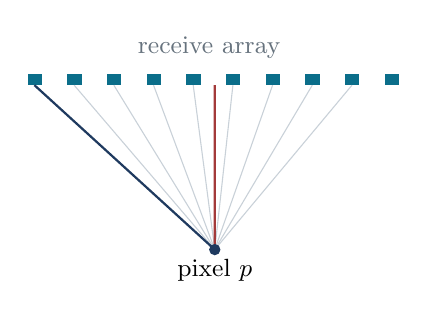
\begin{tikzpicture}[scale=.72]
      \foreach \x in {0,.7,...,6.3}{\fill[Accent] (\x,3.2) rectangle +(.25,.2);}
      \coordinate (p) at (3.3,.3);
      \foreach \x in {.12,.82,...,6.4}{\draw[Rule] (\x,3.2)--(p);}
      \draw[Navy,thick] (.12,3.2)--(p);
      \draw[Warn,thick] (3.3,3.2)--(p);
      \fill[Navy] (p) circle (.1);
      \node[below,font=\small] at (p) {pixel $p$};
      \node[above,Muted,font=\small] at (3.2,3.5) {receive array};
    \end{tikzpicture}

    {\small The echo reaches each element at a different time.}
    \column{.54\textwidth}
    \small
    \vspace{-.5em}
    \[
      \tau_{\rm TX}(p,n)=\min_e\Big(\tfrac{\|p-r_e\|}{c}+t_{0,n,e}\Big)-t_{{\rm init},n}
    \]
    \[
      \tau_{\rm RX}(p,e)=\tfrac{\|p-r_e\|}{c},\qquad k=f_s\big(\tau_{\rm TX}+\tau_{\rm RX}\big)
    \]
    \[
      y_{\rm DAS}(p)=\sum_{n=1}^{21}\sum_{e=1}^{128} a_{n,e}(p)\; s_{n,e}\big(k_{n,e}(p)\big)
    \]
    Non-integer $k=i+\alpha$ is linearly interpolated; samples outside the trace count as zero. $a_{n,e}$ is the F-number apodization window.
  \end{columns}
\end{frame}

% 4 -------------------------------------------------------------- DMAS
\begin{frame}{Delay-multiply-and-sum (DMAS)}
  \small
  DMAS multiplies the delayed channel values in pairs, so a pair counts strongly only when two channels agree:
  \[
    q_{ij}=\operatorname{sign}(s_is_j)\sqrt{|s_is_j|}=u_iu_j,\qquad u_i=\operatorname{sign}(s_i)\sqrt{|s_i|}
  \]
  Direct summation needs $128\cdot127/2=8{,}128$ products per pixel and transmit event. Using $(\sum u_i)^2=\sum u_i^2+2\sum_{i<j}u_iu_j$ and $u_i^2=|s_i|$:
  \[
    \sum_{i<j}u_iu_j=\frac12\Big[\Big(\sum_i u_i\Big)^2-\sum_i|s_i|\Big]
  \]
  \begin{block}{Result}
    Two running sums replace 8,128 products, about 64 times fewer terms. The identity is exact and is applied per transmit event; the 21 event results are then added.
  \end{block}
\end{frame}

% 5 -------------------------------------------------------------- objectives
\begin{frame}{Objectives}
  \begin{enumerate}\setlength\itemsep{.8em}
    \item Implement DAS and DMAS with a CPU double-precision reference.
    \item Optimize the CPU and CUDA implementations.
    \item Check that optimized outputs still match the reference.
    \item Measure the speedup with a clearly defined timing boundary.
  \end{enumerate}
\end{frame}

% 6 -------------------------------------------------------------- dataset
\begin{frame}{Dataset and benchmark setups}
  \begin{columns}[T,onlytextwidth]
    \column{.5\textwidth}
    \small
    \begin{tabularx}{\linewidth}{@{}>{\bfseries}p{2.2cm} X@{}}
      Source & JHU PULSE Lab phantom, Alpinion L3-8\\
      Cases & Hypoechoic cyst; hyperechoic scatterers\\
      Transmits & 21 coherent plane waves\\
      Receive & 128 elements, 0.3 mm pitch\\
      RF samples & 4,352 per channel, float32\\
      Sampling & $f_s=40$ MHz, $f_c=6$ MHz\\
    \end{tabularx}
    \column{.44\textwidth}
    \small
    \begin{block}{Current run}
      $128\times191$ grid, $z=3$--$60$ mm\\
      i7-13700H, RTX 3050 Laptop (6 GB)
    \end{block}
    \begin{block}{Earlier run}
      $507\times600$ grid\\
      i7-10750H, GTX 1650
    \end{block}
    \scriptsize Reported separately; absolute times are not compared across runs.
  \end{columns}
\end{frame}

% 7 -------------------------------------------------------------- methodology
\begin{frame}{Methodology}
  \begin{columns}[T,onlytextwidth]
    \column{.5\textwidth}
    \begin{block}{Verification before timing}
      \small
      \begin{itemize}\setlength\itemsep{.3em}
        \item CPU double-precision reference with an explicit delay model
        \item Unit checks on interpolation and out-of-range samples
        \item Four pixels recomputed in Python from the HDF5 data: max difference $4.46\times10^{-11}$
        \item Whole-image comparison of each optimized variant
      \end{itemize}
    \end{block}
    \column{.44\textwidth}
    \begin{block}{Timing}
      \small
      \begin{itemize}\setlength\itemsep{.3em}
        \item 2 warm-up runs, 30 timed runs, median reported
        \item CPU: \texttt{steady\_clock} around the compute loop
        \item GPU: CUDA events around the kernel
        \item Excluded: file loading, host-to-device copy, envelope and log compression
      \end{itemize}
    \end{block}
  \end{columns}
\end{frame}

% 8 -------------------------------------------------------------- GPU
\begin{frame}{GPU implementation: one thread per pixel}
  \begin{columns}[T,onlytextwidth]
    \column{.36\textwidth}
    \centering
    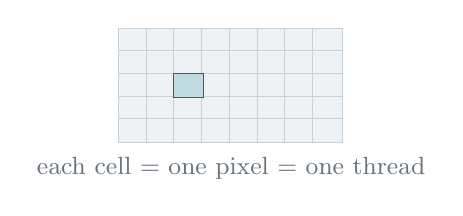
\begin{tikzpicture}[scale=.8]
      \foreach \r in {0,...,4}{\foreach \c in {0,...,7}{
        \node[draw=Rule,fill=LightBg,minimum width=.38cm,minimum height=.3cm,inner sep=0pt] at (\c*.44,-\r*.36) {};}}
      \node[draw=Accent,fill=Accent!25,minimum width=.38cm,minimum height=.3cm,inner sep=0pt] at (2*.44,-2*.36) {};
      \node[below,font=\small,Muted] at (1.55,-1.7) {each cell = one pixel = one thread};
    \end{tikzpicture}
    \column{.58\textwidth}
    \small
    Pixels are independent, so the 24,448 output pixels map directly onto GPU threads. Each thread:
    \begin{enumerate}\setlength\itemsep{.2em}
      \item derives its pixel position $(x,z)$ from its thread index,
      \item finds its receive-element range from the aperture bounds,
      \item loops over those elements and the 21 transmits, interpolating the RF data,
      \item writes one output value.
    \end{enumerate}
    Neighbouring threads read neighbouring samples. The kernels use FP32 (FP64 runs at 1/32 rate on GeForce) and are checked against the FP64 CPU reference.
  \end{columns}
\end{frame}

% 9 -------------------------------------------------------------- opt 1
\begin{frame}[fragile]{Optimization 1: compile-time sizes}
  The probe always has 21 transmits and 128 receivers, but the first code treated them as variables.
  \begin{lstlisting}
// before: runtime sizes
for (tx = 0; tx < n_tx; ++tx)
  for (rx = 0; rx < n_rx; ++rx) ...

// after: template parameters
template <class Real, size_t N_TX, size_t N_RX>
void das_kernel(...);   // <float, 21, 128>
  \end{lstlisting}
  \small The compiler can unroll the loops and keep values in registers. The equation does not change. On its own this gave about 1.0$\times$ on the CPU (earlier run).
\end{frame}

% 10 ------------------------------------------------------------- opt 2
\begin{frame}[fragile]{Optimization 2: compute the receive distance once}
  The pixel-to-element distance does not depend on which transmission is running, but the first code recomputed it for each of the 21.
  \begin{lstlisting}
for (rx in aperture) {
  rx_time = sqrt(dx*dx + z*z) / c;   // once
  for (tx = 0; tx < 21; ++tx)
    sum += interp(raw, (tx_time[tx] + rx_time) * fs);
}
  \end{lstlisting}
  \small Receive-path square roots per pixel drop from 2,688 to 128: about 778 million fewer per frame on the $507\times600$ grid.
\end{frame}

% 11 ------------------------------------------------------------- opt 3
\begin{frame}{Optimization 3: aperture bounds instead of \texttt{acos}}
  \begin{columns}[T,onlytextwidth]
    \column{.56\textwidth}
    \small
    The F-number window ignores elements far to the side of a pixel. The old code computed an angle with \texttt{acos} for every element and skipped the ones outside.

    \smallskip
    The window is $|x-x_e|\le z/(2F)$ and the elements are evenly spaced, so it solves directly for an index range:
    \[
      e_{\min}=\Big\lceil\tfrac{x-z/2F-x_0}{\Delta x}\Big\rceil,\quad
      e_{\max}=\Big\lfloor\tfrac{x+z/2F-x_0}{\Delta x}\Big\rfloor
    \]
    (clamped to $0..127$). The loop runs only over this range: no trigonometry, no per-element branch, and inner-loop iterations fall from 817.7 M to 447.2 M.
    \column{.38\textwidth}
    \centering
    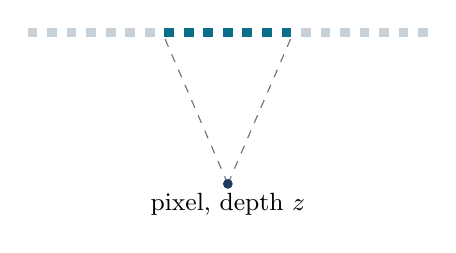
\begin{tikzpicture}[scale=.62]
      \coordinate (p) at (4,0);
      \foreach \i in {0,...,20}{
        \pgfmathsetmacro{\xx}{0.4*\i}
        \pgfmathtruncatemacro{\inside}{abs(\xx-4)<1.31}
        \ifnum\inside=1
          \fill[Accent] (\xx-.1,3) rectangle +(.2,.2);
        \else
          \fill[Rule] (\xx-.1,3) rectangle +(.2,.2);
        \fi}
      \draw[Muted,dashed] (p)--(2.7,3);
      \draw[Muted,dashed] (p)--(5.3,3);
      \fill[Navy] (p) circle (.1);
      \node[below,font=\small] at (p) {pixel, depth $z$};
    \end{tikzpicture}

    {\scriptsize Only highlighted elements are summed.}
  \end{columns}
\end{frame}

% 12 ------------------------------------------------------------- opt 4
\begin{frame}{Optimization 4: cheaper memory access}
  \begin{itemize}\setlength\itemsep{.8em}
    \item \textbf{GPU constant memory.} Element positions and transmit delays are read-only and identical for every thread, so they sit in \texttt{\_\_constant\_\_} memory. When a warp reads one address it is served as a single broadcast.
    \item \textbf{CPU lookup tables.} The lateral term $(x_i-x_e)^2$ and depth term $z_k^2$ are separable, so they are tabulated once instead of recomputed per pixel.
    \item \textbf{Shift indexing.} $N_{RX}=128=2^7$, so multiplying by 128 becomes a left shift by 7 once the size is a compile-time constant.
  \end{itemize}
  \medskip
  {\small The 46.8 MB RF buffer exceeds the 12 MB L3 cache, so on one CPU thread the receive loop (98.2\% of run time) is limited by memory access.}
\end{frame}

% 13 ------------------------------------------------------------- results
\begin{frame}{Results}
  \begin{columns}[T,onlytextwidth]
    \column{.31\textwidth}
    \textbf{\small Current run, DAS (ms)}\\[-.1em]
    {\scriptsize hyperechoic, $128\times191$, RTX 3050}
    \centering
    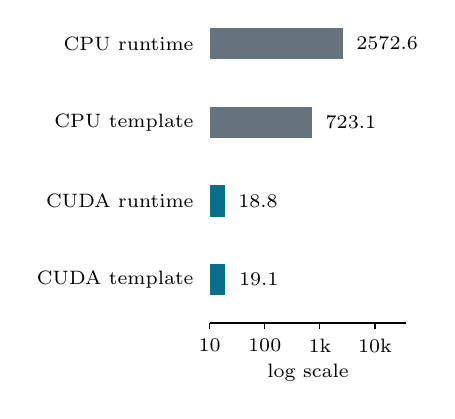
\begin{tikzpicture}[font=\scriptsize]
      \def\xo{1.25}
      \foreach \y/\lab/\ee/\val/\col in {
        3/CPU runtime/2.94/2572.6/Muted,
        2/CPU template/2.55/723.1/Muted,
        1/CUDA runtime/1.44/18.8/Accent,
        0/CUDA template/1.45/19.1/Accent}{
        \node[anchor=east] at (\xo-.08,\y) {\lab};
        \fill[\col] (\xo,\y-.2) rectangle (\ee,\y+.2);
        \node[anchor=west] at (\ee+.05,\y) {\val};}
      \draw (\xo,-.55)--(\xo+2.5,-.55);
      \foreach \t/\l in {0/10,.7/100,1.4/{1k},2.1/{10k}}{
        \draw (\xo+\t,-.55)--(\xo+\t,-.63);
        \node[below] at (\xo+\t,-.63) {\l};}
      \node[below] at (\xo+1.25,-.95) {log scale};
    \end{tikzpicture}

    \raggedright\scriptsize CPU $\to$ CUDA: $137\times$ (hyper.), $153\times$ (hypo.).
    \column{.35\textwidth}
    \textbf{\small Earlier run, naive vs optimized (ms)}\\[-.1em]
    {\scriptsize $507\times600$, GTX 1650, FP32 \texttt{-O3}}
    \centering
    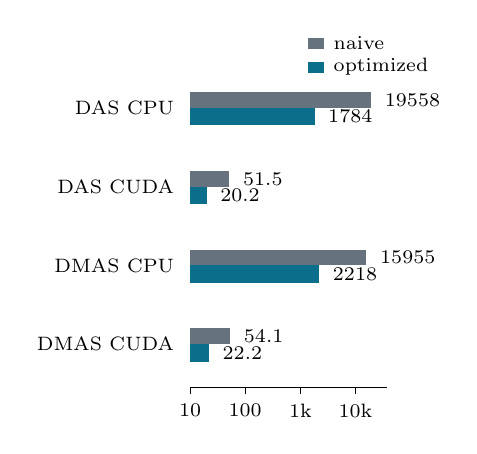
\begin{tikzpicture}[font=\scriptsize]
      \def\xo{1.25}
      \foreach \y/\lab in {3.0/DAS CPU,2.0/DAS CUDA,1.0/DMAS CPU,0/DMAS CUDA}{
        \node[anchor=east] at (\xo-.08,\y) {\lab};}
      \foreach \y/\n/\no/\o/\oo in {
        3.0/2.30/19558/1.58/1784,
        2.0/0.50/51.5/0.21/20.2,
        1.0/2.24/15955/1.64/2218,
        0/0.51/54.1/0.24/22.2}{
        \fill[Muted] (\xo,\y) rectangle (\xo+\n,\y+.2);
        \node[anchor=west] at (\xo+\n+.05,\y+.1) {\no};
        \fill[Accent] (\xo,\y-.22) rectangle (\xo+\o,\y);
        \node[anchor=west] at (\xo+\o+.05,\y-.11) {\oo};}
      \draw (\xo,-.55)--(\xo+2.5,-.55);
      \foreach \t/\l in {0/10,.7/100,1.4/{1k},2.1/{10k}}{
        \draw (\xo+\t,-.55)--(\xo+\t,-.63);
        \node[below] at (\xo+\t,-.63) {\l};}
      \fill[Muted] (\xo+1.5,3.75) rectangle +(.2,.14);\node[anchor=west] at (\xo+1.7,3.82) {naive};
      \fill[Accent] (\xo+1.5,3.45) rectangle +(.2,.14);\node[anchor=west] at (\xo+1.7,3.52) {optimized};
    \end{tikzpicture}
    \column{.29\textwidth}
    \textbf{\small Output agreement}\\[-.1em]
    {\scriptsize hypoechoic, CPU vs CUDA}
    \centering\plot{cpwc_hypoechoic_cpu_cuda_comparison.png}

    \raggedright\scriptsize Correlation 0.9999999996, NRMSE $2.88\times10^{-5}$. CUDA runtime and template outputs are bitwise identical.
  \end{columns}
\end{frame}

% 14 ------------------------------------------------------------- findings
\begin{frame}{Key findings}
  \begin{itemize}\setlength\itemsep{.7em}
    \item One thread per pixel cuts DAS compute time by about 137--153$\times$ against the CPU build on the current grid.
    \item FP32 CUDA output agrees with the FP64 CPU reference (NRMSE $2.9\times10^{-5}$).
    \item CPU gains came from removing redundant work (shared distances, aperture bounds), not from compile-time sizes alone.
    \item Compile-time sizes gave no speedup on the CUDA kernel: whether a change helps depends on the hardware.
    \item With the sum identity, GPU DMAS runs about 2 ms slower than DAS (22.17 vs 20.22 ms, earlier run).
  \end{itemize}
\end{frame}

% 15 ------------------------------------------------------------- conclusion + future
\begin{frame}{Conclusion and future scope}
  \begin{columns}[T,onlytextwidth]
    \column{.47\textwidth}
    \begin{block}{Conclusion}
      \small
      \begin{itemize}\setlength\itemsep{.4em}
        \item DAS and DMAS were implemented with a verified CPU reference and optimized for CPU and CUDA without changing the model.
        \item The largest gain comes from mapping independent pixels to GPU threads; on the CPU, removing redundant work matters most.
        \item Speedups hold for compute time only, not end-to-end frame rate.
      \end{itemize}
    \end{block}
    \column{.47\textwidth}
    \begin{block}{Future scope}
      \small
      \begin{itemize}\setlength\itemsep{.4em}
        \item Confirm the waveform peak-time convention and compare with an independent trusted image.
        \item Measure end-to-end time including transfers, envelope detection and log compression.
        \item Add a multithreaded CPU baseline and repeat timing under controlled load.
        \item Try shared-memory or texture caching of the RF data on the GPU.
      \end{itemize}
    \end{block}
  \end{columns}
\end{frame}

\end{document}
